\documentclass[a4paper,twoside,10pt]{article}
\usepackage{listings}

%
%  Created by Marc Egli on 2011-12-19.
%  Copyright (c) 2011 __MyCompanyName__. All rights reserved.
%
%

% This is now the recommended way for checking for PDFLaTeX:
\usepackage{ifpdf}
\usepackage[utf8]{inputenc}
\usepackage[pdftex]{graphicx} %%Grafiken in pdfLaTeX
\usepackage{amsmath}
\usepackage{amsthm}
\usepackage{amsfonts}
\usepackage{float}
\usepackage{fancyhdr} %%Fancy Kopf- und Fußzeilen
\usepackage{a4wide} %%Kleinere Seitenränder = mehr Text pro Zeile.

\usepackage[pdftitle={Fuchsjagd},%
						pdfauthor={Marc Egli, Tarik Azarnait},%
						pdfcreator={TextMate2},
						pdfsubject={Seminararbeit Mobile Applications},
						plainpages=false,
						pdfpagelabels,
						colorlinks,
						linkcolor=black,
						filecolor=black,
						citecolor=black]{hyperref}


%\newif\ifpdf
%\ifx\pdfoutput\undefined
%\pdffalse % we are not running PDFLaTeX
%\else
%\pdfoutput=1 % we are running PDFLaTeX
%\pdftrue
%\fi

\ifpdf
\usepackage{subfigure}
\usepackage[pdftex]{graphicx}
\else
\usepackage{graphicx}
\fi

\usepackage[ngerman]{babel}
\usepackage[T1]{fontenc}


\begin{document}
\pagestyle{empty} %%Keine Kopf-/Fusszeilen auf den ersten Seiten.
%!TEX root = ../index.tex

\begin{titlepage}
\author{Marc Egli \& Tarik Azarnait} 
\title{Fuchsjagd} 
\date{} 
\begin{center}

\Large
\textsc{Seminararbeit}\\
\textsc{Handheld}\\



\vspace{0.5cm}
\begin{center}
% \includegraphics[width=0.4\textwidth]{Pictures/zDNM_front}
\end{center}
\textsc{Fuchsjagd} 
\vspace{1cm}

\large
Autoren\\
Marc Egli \textsl{eglimar1@students.zhaw.ch}\\
Tarik Azarnait \textsl{azarntar@students.zhaw.ch}\\

\vspace{1cm}
Betreuer\\
Christian Vils\\
\vspace{1.0cm}




\textsc{Herbstsemester 2011}\\
\textsc{Hochschule für Technik Zürich}\\
\vspace{0.5cm}
\normalsize
Copyright \copyright  by Marc Egli \& Tarik Azarnait

\end{center}

\end{titlepage}
\newpage


\pagestyle{fancy} %%Ab hier die Kopf-/Fusszeilen: headings / fancy / ...
\newpage
\tableofcontents
\listoffigures

%!TEX root = ../index.tex

\newpage
\section{Abstract} % (fold)
\label{sec:Abstract}
Es soll das Spiel “Fuchsjagd” welches normalerweise mit Peilsendern und Richtantennen gespielt wird, für Smartphones entwickelt werden welche mit Hilfe von GPS und Kompass den Gebrauch von Funkequipment erübrigen.
Dadurch kann dieses Spiel auch ohne eine Amatuerfunklizenz gespielt werden. Die Applikation sollte auf möglichst vielen Platformen laufen, so dass jeder Teilnehmer mit seinem eigenen Smartphone mitspielen kann.

Grundsätzlich soll die Seminararbeit als eine Einführung in die Smartphone Entwicklung dienen. Da die Anwendung auf möglichst vielen Smartphones benutzbar sein soll, muss dafür eine Technologie (z.B Phonegap) evaluiert und gebraucht werden, welche dies ermöglicht. Als Weiterführung könnte man die Implementation, Vor- und Nachteile auf den spezifischen nativen Technologien prüfen.  

Ziel ist es das Spiel spielbar in einer Smartphone Anwendung implementiert zu haben. Implementationsspezifisch zu evaluierende Punkte sind die Konfiguration für die Spielrunde (z.B. zu suchende Koordinaten setzen), welche direkt gemacht wird im Phone oder über eine administrierende Applikation an die Teilnehmer gesendet werden kann, und das Monitoring, mit dem man möglicherweise den ganzen Spielverlauf auf einer administrierenden Applikation mitverfolgen und nachvollziehen kann.
% section Abstract (end)

Thema: Implementation einer Smartphone Anwendug für das Funkspiel Fuchjagt

\subsubsection{Ausgangslage} % (fold)
\label{ssub:Ausgangslage}
Das Spiel Fuchsjagt benötigt teure und komplizierte Funkgeräte, um mit einem Peilsender und Richtantennen bestimmte Orte zu finden. Es soll eine Anwendung entwickelt werden, welche das Fuchsjagt spielen für einfache Smartphonebesitzer möglich macht.
% subsubsection Ausgangslage (end)

\subsubsection{Ziel der Arbeit} % (fold)
\label{ssub:Ziel der Arbeit}
Das Ziel der Arbeit ist die Entwicklung einer Anwendung, welche das Spielen der Fuchsjagt mittels einem Smartphone ermöglicht. Die Anwendung soll auf möglichst vielen verschiedenen Smartphones brauchbar sein.
% subsubsection Ziel der Arbeit (end)

\subsubsection{Aufgabenstellung} % (fold)
\label{ssub:Aufgabenstellung}
Einarbeiten in das Feld der Smartphone Entwicklung.
Evaluieren einer geeigneten Technologie, um das Requirement der mobilität auf vielen verschiedenen Geräte zu erreichen (z.B. Phonegap)
Entwicklung der Anwendung mit Design, Implementation, Testing auf Iphone 4 und Android 2.3.
Weiterführend:
Aufzeigen der Vor- und Nachteile von nativen Implementationen
Verbesserte Konfiguration über eine administrierende Applikation
Monitoring der Andwender während dem gebraucht der Andwendung.
% subsubsection Aufgabenstellung (end)

\subsection{Erwartete Resultate} % (fold)
\label{sub:Erwartete Resultate}
Eine laufende Smartphoneanwendung die das Spielen von Fuchsjagt ermöglicht.
Eine Dokumentation welche folgende Punte enthält:
\begin{itemize}
    \item Evaluation einer Technologie, welche auf vielen Smartphones anwendbar ist.
    \item Dokumentation der Applikation: Design, Implementation, Testing und Gebrauch der Anwendung.
    \item Weiterführende Themen: Evaluation von nativen Implementationen, Konfiguration und Monitoring einer administrierenden Applikation
\end{itemize}

% subsection Erwartete Resultate (end)

\subsection{Geplante Termine} % (fold)
\label{sub:Geplante Termine}
\begin{itemize}
    \item Kick-Off
    \item Teaser
    \item Zwischenstandsmeeting
    \item Schlusspräsentation HSZ-T
\end{itemize}

% subsection Geplante Termine (end)

%!TEX root = ../index.tex

\newpage
\section{Fuchsjagd Sport} % (fold)
\label{sec:Fuchsjagd Sport}

Unter Fuchsjagd versteht man im Amateurfunk eine Outdoor-Sportart~\cite{bib:amateurfunk_wiki}, die an einen Orientierungslauf erinnert. Dabei sind die Teilnehmer mit tragbaren Funkempfängern ausgestattet, mit denen sie die verschiedenen Anlaufstellen orten können. An diesen zu suchenden Stellen werden Rundstrahlantennen versteckt, welche Signale aussenden.

Dies schafft die Grundlage für den Amateurfunk Orientierungslauf, wobei ein Teilnehmer um das Ziel zu erreichen alle Stationen suchen und anlaufen muss. Als weitere Hilfsmittel hat er zusätzlich eine Karte und einen Kompass. Damit kann er die Ziele mittels der Signalstärke ungefähr ermitteln und sich die Route planen, die nicht vom Spiel vorgegeben ist. 

\subsection{Geschichte} % (fold)
\label{sub:Geschichte}

Bereits in den Zwanzigerjahren spielte man mit Funkgeräten die Fuchsjagd. In den jungen Jahren des Sports spielte man auf einem See wobei man den Fuchs (Sender) in einem Schiff auf ein bestimmtes Ziel zu bewegte. Die Absicht dahinter war es, das Schiff zu finden, bevor es sein Ziel erreichte. Durch die Wellen auf dem Wasser wurde die Peilung jedoch sehr erschwert und so wurde der Fuchs nur mit Glück gefunden.

In den Sechzigerjahren fand das Spiel dann in der heutigen Ausprägung auf dem Land statt, wobei die Sendeanlage in einem Auto in einem Wald versteckt wurde. ~\cite{bib:ardf}
% subsection Geschichte (end)

\subsection{Ausprägungen} % (fold)
\label{sub:Ausprägungen}

Ausser der Fuchsjagd, welche das rasche Finden eines Senders mit Hilfe von Empfänger, Karte und Kompass anstrebt, gibt es noch andere Ausprägungen:

\subsubsection{Foxoring} % (fold)
\label{ssub:Foxoring}
Ein Orientierungslauf mit Zielbereichen, die auf der Karte eingetragen und bekannt sind. In einem solchen Zielkreis angekommen muss der Mitstreiter das genaue Ziel jedoch mithilfe seines Richtfunkempfängers orten.
% subsubsection Foxoring (end)

\subsubsection{Fuchswanderung} % (fold)
\label{ssub:Fuchswanderung}
Eine Fuchsjagd, welche nicht auf Zeit gespielt wird und die Teilnehmer über einen schöne Wanderung in der Natur führt.
% subsubsection Fuchswanderung (end)

\subsubsection{Grossraum-Fuchsjagd} % (fold)
\label{ssub:Grossraum-Fuchsjagd}
Dabei wird ein Fuchs in einem grossen Gebiet versteckt. Für die Teilnahme am Wettbewerb kann man seine durch Peilung geschätzte Position des Fuchs einschicken, wobei die genauste Schätzung gewinnt. Weiter nehmen am Wettbewerb auch mobile Sucher teil, welche versuchen den Fuchs tatsächlich zu finden.
% subsubsection Grossraum-Fuchsjagd (end)
% subsection Ausprägungen (end)

% section Fuchsjagd Sport (end)

%!TEX root = ../index.tex

\newpage
\section{Mobile Applikation} % (fold)
\label{sec:Mobile Applikation}

\subsection{Vorbereitung} % (fold)
\label{sub:Vorbereitung}
\subsubsection{Marktanalyse} % (fold)
\label{ssub:Marktanalyse}
Zur Zeit ist in der Schweiz das iPhone das meist verkaufte Smartphone. Dies und der App Store von Apple sind Gründe, weswegen viele Unternehmen ihre Mobilapplikationen erst für das iPhone entwickeln. Zur Zeit wächst jedoch der Android Markt sehr schnell und wird das iPhone wahrscheinlich vom ersten Platz verdrängen. Das Entwickeln einer App für Android ist jedoch in einigen Punkten komplexer als es für das iPhone ist, da die Diversität der Geräte massiv höher ist und kaum ein Gerät auf einen relevanten Marktanteil kommt. Daher ist es zur Zeit sinnvoll eine Mobile Anwendung für mehrere Geräteklassen zu entwickeln.
% subsubsection Marktanalyse (end)

\subsubsection{Plattformevaluation} % (fold)
\label{ssub:Plattformevaluation}
Da die Verfasser dieser Arbeit iOS und Android Geräte verwenden, wurde auf ein "`Crossplatform Framework"' gesetzt. Zum Zeitpunkt dieser Evaluation gab es zwei mögliche Wege plattformunabhängige Applikationen zu erstellen.
\begin{itemize}
    \item Adobe Flex
    \item PhoneGap
\end{itemize}
Da PhoneGap bessere Unterstützung für exotische Plattformen hatte und es mit JavaScript auf einer Programmiersprache beruht, welche auch im World Wide Web eingesetzt wird und Adobe Flex mit ActionScript3 auf eine Sprache setzt, welche ausser in Adobe Produkten nicht eingesetzt wird, fiel die Entscheidung auf PhoneGap.
% subsubsection Plattformevaluation (end)
% subsection Vorbereitung (end)

\subsection{Geolocation Native Feature} % (fold)
\label{sub:geolocation_native_feature}
Von den Geolocation Native Funktionen werden zwei PhoneGap Methoden verwendet. Initial wird getCurrentPosition verwendet um die aktuelle Position festzustellen. Danach werden mit watchPostion Veränderungen festgestellt und abgespeichert. Die Ankunft von neuen Geolocation Daten löst immer direkt eine Berechnung der Abstände und Richtungen zu den Zielen aus. Der Wert den die Methoden zurückliefern ist die Gradangabe unterschiedlich von Nord. Daher ist Ost 90, Süd 180 und West 270.
% subsection geolocation_native_feature (end)

\subsection{Kompass Native Feature} % (fold)
\label{sub:kompass_native_feature}
Von der Kompass Native Funktion werden zwei PhoneGap Methoden verwendet. Mit getCurrentHeading wird die initiale Richtung festgestellt. Weiter wird mit watchHeading die Ausrichtung aktualisiert. Die Aktualisierung funktioniert in zeitlich bestimmten Abständen. Die Messungen sollten unter 500 Millisekunden sein um eine flüssige Applikation zu haben. Es ist jedoch darauf zu achten, das die Verarbeitungszeit nicht unterschritten wird, damit man nicht in Probleme mit zu vielen Verarbeitungen hinein läuft. Ein Update der Kompass-Daten löst immer eine Kalkulation der Signal-Stärke aus, welche im Zusammenhang mit der Richtung des Ziels (siehe Kapitel~\ref{sub:geolocation_native_feature}) und eingehenden Kompass-Richtung steht.
% subsection kompass_native_feature (end)

\subsection{Kalkulation} % (fold)
\label{sub:kalkulation}
\subsubsection{Richtung} % (fold)
\label{ssub:richtung}
Die Richtung wird mittels dem Öffnungswinkel zwischen den zwei Punkten berechnet und in Abhängigkeit zu Nord gebracht. So erhält man eine Richtung wie es die Kompass Native Funktion zurück liefert. Diese können dann direkt verglichen werden um die Korrektheit der Richtung und somit die Signalstärke ~\ref{ssub:signalstärke}
 festzustellen. 
% subsubsection richtung (end)
\subsubsection{Signalstärke} % (fold)
\label{ssub:signalstärke}
Die Signalstärke wird angezeigt, wenn die eigene Richtung näher als 100 Grad an der Richtung des Ziels ist. In einer ersten Implementation wurde die Stärke linear berechnet. Daher: Wenn die Richtung um 99 Grad daneben war wurde 1\% Signalstärke angezeigt, bei 50 Grad waren es 50\% Signalstärke. In einem zweiten Schritt wurde die Signalstärke dann exponentiell berechnet. Daher: Bei kleiner Richtungsänderung in der nähe der perfekten Ausrichtung verändert sich die Signalstärke sehr stark, bei grösseren Richtungsänderungen im Bereich von 100 Grad Abweichung des Ziels verändert sich die Signalstärke nur schwach. Dieses Verhalten ist auch bei der Richtfunk-Fuchsjagd der Fall. Die Grösse mit den 100 Grad Abweichung kann mit einer guten Richtfunk Anlage ebenfalls bewerkstelligt werden. Schlechtere Anlagen haben einen grösseren Radius wo das Signal angezeigt wird und somit wird in allen Richtungen ein stärkeres oder schwächeres Signal festgestellt.
% subsubsection signalstärke (end)
\subsubsection{Distanz} % (fold)
\label{ssub:distanz}
Die Distanz wird mit einer Hypotenuse zwischen den beiden Punkten (Eigene Position und Ziel) mit den Deltas der Längen- und Höhenbreite berechnet. 
% subsubsection distanz (end)
% subsection kalkulation (end)

\subsection{Backend Kommunikation} % (fold)
\label{sub:backend_kommunikation}
Die Backend Kommunikation wurde längere Zeit mit statischen Zielen simuliert. Später sind dann die Daten zu den Zielen mit JSONP Requests vom Backend heruntergeladen worden. JSONP musste verwendet werden um das Problem von Cross Site Referenzen aus Java Script zu lösen, welches aus Security Gründen mit einfachem AJAX nicht machbar ist. Zurückgeliefert wird ein Java Script Array aus dem JSON Object.
% subsection backend_kommunikation (end)

\subsection{Stärkenanzeige} % (fold)
\label{sub:stärkenanzeige}
Für die Anzeige der Signalstärke für x Ziele wurde dynamisches HTML verwendet, was grundsätzlich keine schöne Lösung ist. Dabei werden mittels Java Script HTML Tags nach dem Laden für jedes gefundene Ziel ein HTML-Div in einen schon vorhandenen div eingebunden. Dabei erhält jeder der Divs eine individuelle dem Ziel angepasste ID damit die Signalstärke bei Änderungen angepasst werden kann. Die Signalstärke wird von der Kalkulation in Prozent geliefert. Diese Prozentzahl kann dann direkt im HTML Signalstärke Tag width eingegeben werden, das die prozentuale Grösse vom darum liegenden Tag annimmt.
% subsection stärkenanzeige (end)

\subsection{Datenmanagement} % (fold)
\label{sub:datenmanagement}
Um die Daten der Ziele zu managen, wurde Objekt Orientiertes Java Script verwendet. Ein Ziel besitzt einen Namen, eine fixe Position, welche vom Backend geliefert wird, eine veränderliche Richtung und Entfernung. Zusätzlich besitzt das Objekt zwei Methoden. Die erste wird aufgerufen, wenn sich die eigene Position verändert. Sie berechnet die Distanz und Richtung und speichert diese dann direkt im Ziel-Objekt ab. Die zweite Methode wird aufgerufen, wenn sich die eigene Richtung verändert. Sie berechnet und liefert die neue Signalstärke direkt an den Aufrufer zurück. 
% subsection datenmanagement (end)

\subsection{Design} % (fold)
\label{sub:design}
Die dieser Arbeit vorliegende Applikation (siehe Screenshots) ist nicht mit Design ausgestattet. Zu oberst werden die eigene Längen- und Breitengrade angezeigt. Darunter die eigene Richtung in Abweichung von Nord. 
Im unteren Teil der Applikation befindet sich eine Liste der Ziele, welche grün eingefärbt die Signalstärke für jedes Ziel anzeigt. Das Design soll in naher Zukunft angepasst werden, damit die Applikation ansprechender wird.
% subsection design (end)

\begin{figure}[H]
	\centering			      
        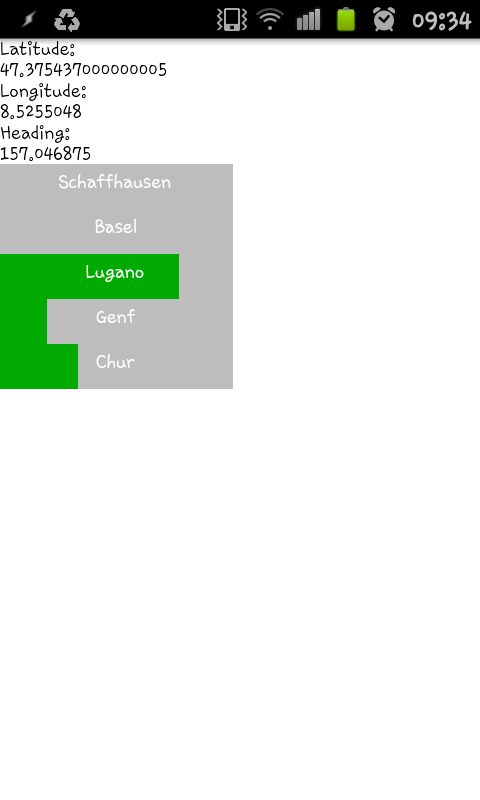
\includegraphics[scale=0.50, trim=0mm 15cm 0mm 0mm, clip]{images/screenshot-1.png}\\
		\caption{Screenshot}
	\label{fig:screenshot-1}
\end{figure}

\subsection{Mini-Kompass} % (fold)
\label{sub:mini_kompass}
Wie im Kapitel Design~\ref{sub:design} beschrieben, ist das Design und Frontend noch nicht ausgereift. Zusätzlich zu den Signalstärken zu den einzelnen Zielen, soll ebenfalls ein kleiner Kompass auf dem Bildschirm angezeigt werden. Dieser ist in der jetzigen Lösung nur als Grad Zahl in Abweichung von Nord angegeben. Somit braucht es für das Spielen der Fuchsjagd lediglich noch eine Karte, die in Papierform den Vorteil der Übersicht und der Beschreibbarkeit hat.
% subsection mini_kompass (end)

\begin{figure}[H]
	\centering			      
        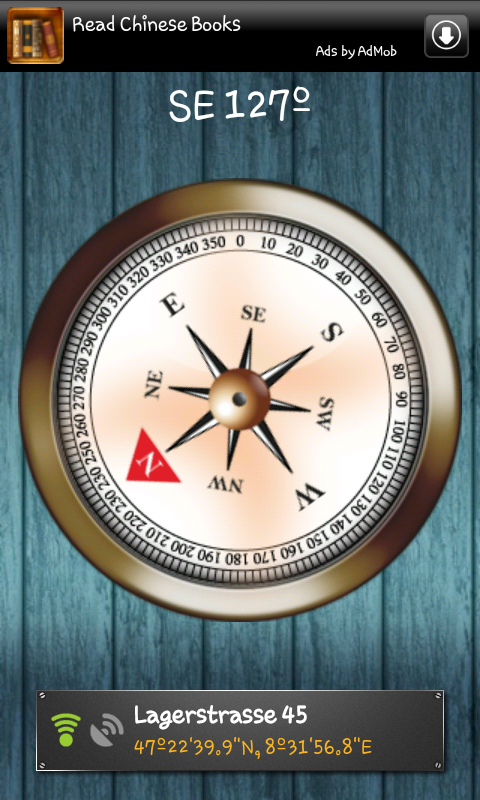
\includegraphics[scale=0.35, trim=5mm 6cm 5mm 6cm, clip]{images/kompass.png}\\
		\caption{Kompass}
	\label{fig:kompass}
\end{figure}
% section mobile applikation (end)

%!TEX root = ../index.tex

\newpage
\section{PhoneGap} % (fold)
\label{sec:PhoneGap}
PhoneGap bietet eine Applikationsplatform auf HTML 5 und CSS 3 Basis. Der Vorteil ist, das die nativen APIs mittels HTML und JavaScript implementiert werden können und dann je nach darunterliegendem Gerät angesprochen werden. Dadurch ist die Codebase der Applikation für alle Geräte die gleiche. Sie wird dann noch in eine standardmässige, geräte- und versionsspezifische Umgebung eingehängt und so auf den Smartphones installiert.

\subsection{PhoneGap Programmierung} % (fold)
\label{sub:PhoneGap Programmierung}

\subsubsection{PhoneGap Android} % (fold)
\label{ssub:PhoneGap Android}
Der einfachste Einstieg in die App Entwicklung mit PhoneGap ist mittels Eclipse. Unter anderem weil es für die anderen IDEs nicht einfach ist Dokumentation mit PhoneGap zu finden. Nachdem Eclipse mit dem Android SDK Plugin ausgestattet worden ist, kann man ein einfaches Android Projekt öffnen, welches ein erstes "`Hello World"' setup im Standard Native Android Style enthält. 
An diesem Standard Projekt muss man nun eine Hand voll Änderungen vornehmen bis man mit der eigentlich Programmierung anfangen kann:
\begin{itemize}
    \item Die phonegap.jar Java Archiv Datei muss in den Ordner für anzuziehende Archive kopiert werden.
    \item Zwei XML Dateien mit Konfiguration müssen in den Ressourcen Ordner kopiert werden. 
    \item In der Standard "`Activity"', einem Baustein einer Nativen Android Applikation, welche bei der Projekt generation mit generiert wurde, muss der standardmässige setContentView() Aufruf mit dem Laden der initialen html Datei ersetzt werden.
    \item Ausserdem müssen im Standard AndroidManifest.xml Einträge wie Permissions, welche die Applikation auf die Features des Android Phones hat, und eine zusätzliche "`Activity"' konfiguriert werden.
    \item Als letztes braucht es noch die phonegap.js Datei, welche in den www Ordner kopiert wird, in welchem dann auch die Applikation oder Web-Content, hinkommt.
\end{itemize}
Das Setup kann mit einem einfachen "`Hello World"'-html im www Ordner überprüft werden. Mit der Run... Taste und dem neuen Aufsetzten einer "`Android Applikaton"' wird die "`Hello World"' Seite einfach auf dem Android-Phone oder dem Android Emulator angezeigt.
% subsubsection PhoneGap Android (end)

\subsubsection{Zugriff auf ein richtiges Android Phone} % (fold)
\label{ssub:Zugriff auf ein richtiges Android Phone}
Der Zugriff von Eclipse oder anderen IDEs auf ein Android Phone ist sehr einfach. Dazu muss lediglich in den Einstellungen auf dem Gerät unter Applikationen das Debug-Flag einschalten. Danach das Telefon mit dem USB Kabel an den Computer anhängen und beim laufen lassen einer Applikation erscheint es dann zur Auswahl in der Liste. Die Applikation wird dann deployed und installiert, und ist danach auch ohne Verbindung zum Computer verfügbar.
% subsubsection Zugriff auf ein richtiges Android Phone (end)

\subsubsection{Android Emulatoren} % (fold)
\label{ssub:Android Emulatoren}
Die Emulatoren, welche das Android SDK zu Verfügung stellt sind für einfache "`Hello World"' Appliktionen mehr als passable. Die Geschwindigkeit lässt jedoch schon beim Aufstarten von einem MacBook zu wünschen übrig. Der Angezeigte Android Desktop ruckelt und es dauert lange bis Klicks beantwortet werden. Wenn Andoid Native Features wie Geolocation oder der Kompass angesprochen werden sollen, muss dies zuerst kompliziert konfiugriert werden, wie es vielen Foren im Internet zu entnehmen ist. HTML5 und JavaScript funktionieren. Somit können die Emulatoren für einfache Regression Tests nützlich sein. Bei komplexeren Applikationen sollte man für das Programmieren jedoch ein richtiges Android Phone zur Verfügung haben wo man die Tests schnell und einfach darauf deployen und testen kann.
% subsubsection Android Emulatoren (end)

\subsubsection{Debuggen mit Eclipse} % (fold)
\label{ssub:Debuggen mit Eclipse}
Bei angehängtem Android Phone, können alle Aktivitäten im Eclipse angezeigt werden. Java Code könnte auch genau gedebugged werden. Leider können HTML und Java Script nicht gedebugged werden. Die Debug-View zeigt jedoch die Fehler wie einem Browser jedoch in chronologischem Ablauf zusammen mit den Warnings und Infos vom Phone (Klicks, Laden, etc). Somit kann dies dennoch hilfreich sein. 
% subsubsection Debuggen mit Eclipse (end)

% subsection PhoneGap Programmierung (end)
% section PhoneGap (end)

\newpage
\section{Server} % (fold)
\label{sec:Server}

\subsection{Einleitung} % (fold)
\label{sub:Einleitung}
Um einen OL einfach durch einen neuen zu ersetzen, wird ein zentraler Webserver verwendet. Das sogenannte Backend vereifacht die Erstellung von OL indem es ermöglicht solche über ein Webformular einzutragen.
% subsection Einleitung (end)

\subsection{Technologie} % (fold)
\label{sub:Technologie}
Da das Backend nicht zentraler Bestandteil dieser Arbeit ist, wurde hier auf schon vorhandene Kenntnisse der Programmiersprache Python und auf Erfahrungen mit dem Django Framework aufgebaut.\\
Django ist ein weit verbreitetes Webframework, welches sich zusammen mit Piston gut für ein solches Projekt eignet.
% subsection Technologie (end)

\subsection{Hosting Evaluation} % (fold)
\label{sub:Hosting Evaluation}
Da Django Applikationen nicht auf jedem Webserver ohne weiteres lauffähig sind, und ein kostenarmer Betrieb auch nach dem Abschliessen dieser Arbeit erzielt werden soll, wurden hier die Bestehenden Applikationshoster ins Auge gefasst.

\subsubsection{Google App Engine} % (fold)
\label{ssub:Google App Engine}
Google betreibt mit der App Engine einen Dienst welche sehr gut Skalierbar ist und für kleine Datenaufkommen auch gratis ist.\\
Jedoch unterstützte die App Engine zu Beginn dieser Arbeit noch keine Relationale Datenbank, was den Programmieraufwand betrachtlich erhöht hätte.
% subsubsection Google App Engnine (end)

\subsubsection{Heroku} % (fold)
\label{ssub:Heroku}
Heroku ist vor allem durch seinen Rails Hosting Service bekannt geworen. Jedoch ist es nun auch möglich diverse andere Frameworks und Sprachen über eigene Scripte einzubinden. Jedoch war dies zu Beginn dieser Arbeit noch nicht so ausgereift und basierte teilweise auf nicht für produktiv Umgebungen konzipierten Anwendungen.
% subsubsection Heroku (end)

\subsubsection{Djangy} % (fold)
\label{ssub:Djangy}
Dieser vielversprechende Service wurde leider kurz vor dieser Arbeit eingestellt, da die Betreiber sich dagegen entschieden haben, Geld aufzunehmen um schneller wachsen zu können.
% subsubsection Djangy (end)

\subsection{ep.io} % (fold)
\label{sub:ep.io}
ep.io ist seit langer Zeit in der Beta Phase und ist nur mit einer persönlichen Einladung nutzbar, jedoch lässt sich ep.io gut mit dem oben aufgeführten Djangy Service Vergleichen. Ein weiterer Vorteil gegenüber App Engine und Heroku ist, dass sich ep.io auf Django Hosting und nicht Web Applikationen im Allgemeinen spezialisiert hat.
% subsection ep.io (end)

% subsection Hosting Evaluation (end)

\subsection{Hosting Entscheidung} % (fold)
\label{sub:Hosting Entscheidung}
Da Marc Egli nach über einem halben Jahr wartezeit noch rechtzeitig als Tester von ep.io zugelassen wurde und ep.io für unsere Zwecke gratis ist, haben wir uns dafür entschieden ep.io zu auszuprobieren.
% subsection Hosting Entscheidung (end)
% section Server (end)
\newpage
\section{Verwendete Tools} % (fold)
\label{sec:Verwendete Tools}

\subsection{TextMate} % (fold)
\label{sub:TextMate}
Der Texteditor Textmate wurde für den HTML/Javascript Teil und für das Schreiben der Dokumentation.
% subsection TextMate (end)

\subsection{Xcode} % (fold)
\label{ssub:Xcode}
Mit Xcode wurde die iPhone App gebundelt.
% subsubsection Xcode (end)
% section Verwendete Tools (end)
%!TEX root = ../index.tex

\newpage
\section{Fazit} % (fold)
\label{sec:Fazit}

Als erstes Positivfazit ist zu betonen, dass das Zeitmanagement in dieser Arbeit sehr gut aufgegangen ist und sich im Vergleich zu früheren Arbeiten sehr verbessert hat. Gute Absprache und speditive Arbeit hat zu einer effizienten Seminararbeit geführt.\\
Die getroffenen Entscheidungen, die gut überdacht und ausgeklügelt waren, haben sich als gute Wahl herausgestellt. Mit PhoneGap konnte die Smartphone Applikation einfach und effizient implementiert werden, Jangy und ep.io sind sehr top of the art Werkzeuge, welche dazu verwendet wurden um einen einfachen Backend Server aufzubauen. LaTeX hat sich als einfache und saubere Lösung für die Dokumentation dieser Arbeit herausgestellt.\\
Es war eine interessante Erfahrung eine Applikation zu sehen, welche auf iOS und Android ohne grosse Anpassungen zum Laufen gekommen ist. Probleme beim IPhone waren das Deployment - wenn auch nur zu Testzwecken. Beim Android war die Schwierigkeit initial die nativen Features Geolocation und Kompass zum Laufen zu bringen. Die Entwicklungsumgebungen sind grundsätzlich für beide Systeme einfach zu installieren und aufzusetzen. 

% section Fazit (end)

\end{document}

